\documentclass[sigconf,authordraft]{acmart}

\usepackage{gensymb}
\usepackage[inline]{enumitem}
\usepackage{amsmath}
\usepackage{graphicx}

\AtBeginDocument{%
  \providecommand\BibTeX{{%
    \normalfont B\kern-0.5em{\scshape i\kern-0.25em b}\kern-0.8em\TeX}}}

\citestyle{acmauthoryear}

\begin{document}

\title{Application of Reinforcement Learning in NASA Swarmathon Competition}

\author{Rolando J. Nieves}
\email{rolando.j.nieves@knights.ucf.edu}
\authornotemark[1]
\affiliation{%
  \institution{University of Central Florida}
  \streetaddress{4000 Central Florida Blvd.}
  \city{Orlando}
  \state{Florida}
  \postcode{32816}
}

\renewcommand{\shortauthors}{Nieves}

\begin{abstract}
  The NASA Swarmathon competition domain provides an excellent proving ground
  for the implementation of multi-agent cooperative behavior using Reinforcement
  Learning (RL). This report documents the results of a study aimed at replacing
  the fixed, swarm-like logic offered as a baseline to competition entrants with
  a system that can be trained in a simulated environment prior to deployment
  onto an entrant's physical robots.
\end{abstract}

\begin{CCSXML}
  <ccs2012>
    <concept>
      <concept_id>10010147.10010178.10010219.10010220</concept_id>
      <concept_desc>Computing methodologies~Multi-agent systems</concept_desc>
      <concept_significance>500</concept_significance>
    </concept>
    <concept>
      <concept_id>10010147.10010257.10010258.10010261.10010275</concept_id>
      <concept_desc>
        Computing methodologies~Multi-agent reinforcement learning
      </concept_desc>
      <concept_significance>500</concept_significance>
    </concept>
  </ccs2012>
\end{CCSXML}

\ccsdesc[500]{Computing methodologies~Multi-agent systems}
\ccsdesc[500]{Computing methodologies~Multi-agent reinforcement learning}

\keywords{multi-agent systems,machine learning,reinforcement learning}

\begin{teaserfigure}
  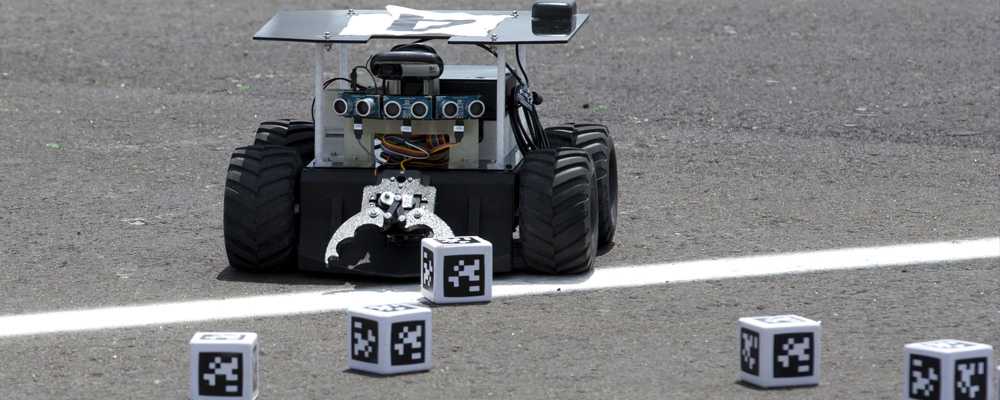
\includegraphics[width=\textwidth]{images/swarmathon-teaser.jpg}
  \caption{Montgomery College ``Swarmie'' in 2017 NASA Swarmathon}
  \Description{Image of a robotic member of the Montgomery College Swarmathon team entrant competing in NASA Swarmathon 2017}
  \label{fig:teaser}
\end{teaserfigure}

\maketitle

\section{Introduction}\label{sec:intro}
The study of applying Reinforcement Learning (RL) into cooperative multi-agent
systems remains a hot topic at the time of this writing. The topic's popularity
owes primarily to the fact that, unlike single agent RL, no single system
architecture has yet emerged as clearly superior among all available options.
Current architectural patterns such as Independent Learners (IL) and
Joint-Action Learners (JAL) exhibit traits that in some environments prove
quite beneficial. In other environments, however, these same traits represent
intolerable liabilities.

Thus, the search for a ``better mouse trap'' in the area of cooperating,
multi-agent RL has led to a proliferation of problem domains under which
methodology performance can be tested and quantified. From grid-world like
synthetic predator-prey scenarios, to more flexible environments like RoboCup
2D Simulated Soccer, these domains offer efficient ways to test theories. One
shortcoming of these problem domains, however, is the difficulty of implementing
any realized achievements into a physical domain.

The NASA Swarmathon problem domain offers an exciting opportunity for research
in this field. This is so because, combined with a robust simulation environment
based around the Robot Operating System (ROS) software suite, the domain offers
a clear path to implementation into physical robots participating in live
competition.

\section{Problem Domain}\label{sec:prob_domain}
In a generic sense, NASA Swarmathon is a resource gathering exercise using a
swarm of autonomous robots. The robotic swarm is expected to gather a set of
resources from their surrounding environment onto a collection area without
relying on any human supervision. NASA's intent with the competition is the
development of technologies that could one day be used to deploy ``advance
missions'' that perform as much preparation as possible at a planetary body site ahead of the arrival by human explorers.

NASA defines the Swarmathon competition environment using the following
elements:

\begin{itemize}
  \item A $16 \times 16$ or $32 \times 32$ meter square field where the
  competition takes place. The field size varies based on the round the
  competition is at.
  \item A swarm of three or six robots, with each robot labeled as a
  ``swarmie.''
  \item Up to 256, $2 \times 2 \times 2$ inch cubes bearing ``April Tag''
  markers on all six faces, known as April Cubes.
  \item A $1 \times 1$ meter square collection area within the competition
  field, known as a ``nest.''
\end{itemize}

During a competition round, a set of April Cubes are randomly strewn across
open areas of the competition field (i.e., no cubes initially start at
the ``nest''). The robotic swarm is then tasked with collecting the cubes onto
the ``nest.'' The periphery of the nest is labeled using another set of ``April
Tags,'' serving as a visual indicator for the robots. Collected cubes must be
in contact with the ``nest'' in order for them to count towards the team's
overall score.

Team members are not allowed contact or communication with the robots
(``swarmies'') during a round, leaving the robots to complete the task
leveraging their built-in sensor package and logic deployed to them prior to the
round. Individual robots are, however, allowed to communicate amongst
themselves. Although no restrictions on underlying physical communication fabric
exists as of this writing, the selected physical fabric must be exposed to the
robots via the ROS Publish-Subscribe communication system. A popular choice among teams is the use of Wi-Fi networking to implement robot-to-robot communication. No restrictions regarding bandwidth or reliability is imposed on the teams as of this writing.

The elements that comprise the ``swarmie'' sensor package include the
following:

\begin{itemize}
  \item Three ultrasonic range finders able to detect obstacles up to 3 meters
  away. The sensors are located in front of the robot, and evenly distributed
  across a $60^{\circ}$ arc.
  \item One Inertial Measurement Unit (IMU) used to estimate robot orientation
  and, in combination with other sensors, robot pose in the fixed competition
  area.
  \item One camera emitting color $320 \times 240$ resolution images at about
  six frames per second (FPS).
  \item One Global Positioning Satellite (GPS) receiver emitting latitude and
  longitude readings that, in combination with other sensors, help establish the
  robot's pose in the competition area.
  \item One odometer emitting wheel movement that, in combination with other
  sensors, help establish the robot's pose in the competition area.
\end{itemize}

In order to combine, or ``fuse,'' several of the sensor readings into a complete
robot pose, the baseline software provided by NASA includes an Extended Kalman
Filter (EKF) pipeline that eventually produces the following pose information:

\begin{itemize}
  \item Cartesian $(x,y,z)$ position with (albeit mostly static) altitude.
  \item Yaw with respect to a fixed reference frame.
  \item Linear $(x,y)$ velocity.
  \item Angular velocity about the Yaw axis
  \item Linear $(x,y)$ acceleration. 
\end{itemize}

Given that the robots are four-wheeled traversing a flat area, linear velocity
and acceleration in the altitude $z$ axis, as well as angular position and
velocity about the Roll and Pitch axes is not calculated.

The NASA baseline software also includes computer vision facilities that, when
combined with the camera and robot pose calculations, are able to provide
information about any ``April Tags'' visible within the robot's field of view.
As stated previously, the April Cubes that the robots must gather are
labeled on all six faces with the aforementioned tags, as is the ``nest''
periphery where the robots must deposit the cubes.

The NASA baseline software is written in terms of the facilities and services
provided by ROS, particularly when it comes to communication. Software provided
by teams must run within ROS and, again, may only utilize the Publish-Subscribe
system provided with ROS for their communication needs. In addition, the NASA
baseline software provides a simulation environment that combines ROS Gazebo
with 3D models of the robots and sensor emulation. During a simulation session,
the communication traffic fed as input to the software components that combine
to implement a robot's logic is practically indistinguishable from traffic that
would be produced by the sensor package of a physical robot.

\section{Related Works}\label{sec:related_works}
Related works notes:

Found an interesting thesis discussing some alternatives to $\epsilon$-greedy exploration/exploitation techniques \cite[pp. 54]{nissen2007large}. The original intent was to find implementation hints for SARSA($\lambda$) but the aforementioned section could be applicable.

Found what could be a good C++ library that provides an implementation of several reinforcement learning algorithms, including SARSA($\lambda$): \cite[RLLib]{samindaa-rllib}. One thing that is a concern is that it uses linear approximation instead of ANNs.

\section{Methodology}\label{sec:methodology}

\subsection{Challenges}\label{subsec:challenges}
There are many aspects of the NASA Swarmathon domain that pose a challenge against the implementation of a Reinforcement Learning (RL) based solution. Chief among these challenges are:

\begin{itemize}
  \item Although the number of April Cubes the Swarmies are tasked with foraging is fixed and known, their exact location in the arena is not.
  \item The Swarmies identify the location of April Cubes using two-dimensional cartesian coordinates $\textbf{L} \in \mathbb{R}^2$ based on the coordinate reference frame individually maintained by each Swarmie.
  \item The Swarmies navigate the competition area primarily using waypoints that are specified as two-dimensional cartesian coordinates $\textbf{W} \in \mathbb{R}^2$, again based on the individual reference frame maintained by each Swarmie.
  \item The Swarmies are not designed to properly map the competition area, thus they are required to continuously detect and properly react to the area's boundaries as well as the collection ``nest.''
\end{itemize}

Addressing each one of the aforementioned challenges is not impossible, but does impact the RL-based solution in ways that could introduce some margin of error and uncertainty.

The lack of persistent mapping capability by the Swarmies is not too difficult a challenge, as both the robot's sensor package and competition area markings make it possible to navigate without having to resort to a map or known landmark locations. The baseline NASA Swarmathon software code contains low-level logic that enables
\begin{enumerate*}[label={(\arabic*)}]
  \item the detection and avoidance of physical obstacles,
  \item the detection of the collection zone (i.e., the ``nest''), and
  \item the detection and avoidance of the competition area boundary.
\end{enumerate*}
Thus, given that hazard avoidance is not the main focus of this RL-based solution, integrating the existing logic is the most efficient course of action to address the challenge.

Considered in isolation, the requirement that the robotic swarm find the location of all the April Cubes with very little prior knowledge is not a very difficult problem. Indeed, such a problem closely resembles a run-of-the-mill mapping exercise. The complications begin to arise once the following facts are taken into consideration:

\begin{itemize}
  \item Each Swarmie calls out the location of each April Cube observed in the competition area using real-space coordinates based on the robot's individual reference frame.
  \item The reference frame maintained by each Swarmie centers its origin at the robot's starting location.
  \item Even with sensor fusion, the reported location by each Swarmie varies by as much as $\pm 0.5$ meters with each sensor reading.
\end{itemize}

The presence of multiple reference frames can be addressed via the use of a simple affine transform to a global reference frame. Given that, at the start of a simulated run, the location of each Swarmie is specified in such a global reference frame, the parameters for such a transform (which would only include a translation component) can be easily communicated to each robot.

The use of real-space coordinates, combined with the variability introduced by the sensor package, makes it nearly impossible to properly attach a true location for an individual April Cube, even after applying a global reference frame transform. Although a system could be devised that could combine multiple observations with SLAM-like techniques to narrow the sensor variability, such is not the focus of this study.

Instead, a more economical approach involves the discretization of the competition area, making it resemble a ``grid world,'' at least for the purposes of April Cube mapping. Given the perceived position variability, at least as produced by sensor fusion, a good starting point for a grid world cell size could be $0.5 \times 0.5$ meters square. Making the grid world cell size into a hyper-parameter of the model makes it possible to supplement the optimization options of the resulting system.

Since in almost all cases the grid world cell size will be far larger than the surface area occupied by an individual April Cube, there exists a very good possibility that multiple cubes will occupy a particular cell. Thus, even after discretization, uniquely attaching a location for each cube remains elusive. However, given that the total number of cubes present is known to each robot, it is possible to indirectly attach a state label to the cubes present in the competition area. Consider that, at any one time, April Cube subsets could be incorporated into one of four mutually-exclusive states:

\begin{description}
  \item[At-Large]: Cubes that are known to exist, but whose location remains unknown.
  \item[Located]: Cubes that are known to be occupying a cell in the competition area grid world, outside of the collection zone.
  \item[In-Transit]: Cubes being transported by Swarmie robots to the collection zone.
  \item[Collected]: Cubes known to be present in the collection zone.
\end{description}

Given that the subsets are mutually exclusive, a simple mathematical relation can be drawn from their individual membership sizes. Let $N$ be the total number of cubes known to exist, $B_u$ be the number cubes considered \textbf{At-Large}, $B_l$ be the number of cubes considered \textbf{Located}, $B_t$ be the number of cubes considered \textbf{In-Transit}, and $B_c$ be the number of cubes considered \textbf{Collected}. Equation \ref{eq:cube_count_relation} depicts the mathematical relation.

\begin{equation}\label{eq:cube_count_relation}
  N = B_u + B_l + B_t + B_c
\end{equation}

The count of April Cubes considered \textbf{In-Transit} or \textbf{Collected} is pretty self-explanatory. The count of cubes considered \textbf{Located} ($B_l$) is a little more nebulous. Given the conditions that led to the discretization of the competition area, not every individual cube spotted by a Swarmie robot will be immediately accounted for in $B_l$. A more apt description for the set would be the number of competition area grid cells known to be occupied by at least one ``April Cube.'' Thus, during most of the competition run, $B_l$ will under-estimate the number of cubes spotted by Swarmies. Fortunately, the combination of the known total cube count ($N$), Equation \ref{eq:cube_count_relation}, and the \textbf{At-Large} set size ($B_u$) help to ensure that any located cube under-count is eventually rectified. Once a grid world cell is considered ``unoccupied'' (e.g., due to a cube in the cell being picked up), the spotting of another cube in the same cell will transition a cube from \textbf{At-Large} to \textbf{Located} (i.e., bump $B_l$ at the expense of $B_u$). Such transitions help lift the ``fog of war'' that obfuscates the location of April Cubes. manifested by the $B_u$ term in Equation \ref{eq:cube_count_relation}.

\subsection{State Space Definition}\label{subsec:state_space}
The set sizes in Equation \ref{eq:cube_count_relation} serve as an excellent starting point for defining the state space that the Reinforcement Learning algorithm in this Swarmathon solution uses. The first four elements in the state space vector \textbf{S} are directly proportional to the set size magnitudes in Equation \ref{eq:cube_count_relation}. In order to broaden the applicability of the learned policy, the state space elements are normalized using the total block count $N$, as shown in Equation \ref{eq:state_space_0_3}. Doing the normalization will allow for the learned policy to be used with any number of total April Cubes.

\begin{equation}\label{eq:state_space_0_3}
  \begin{aligned}
    S_0 &= B_u \div N \\
    S_1 &= B_l \div N \\
    S_2 &= B_t \div N \\
    S_3 &= B_c \div N
  \end{aligned}
\end{equation}

The rest of the state space elements are directly related to the number of Swarmie robots participating in a competition run. As such, the size of the state space vector varies depending on the number of robots competing. Consequently, the learned policy produced in a training session is not portable across scenarios with different Swarmie robot counts. In the context of the NASA Swarmathon competition this is important, since all but the final match are run using three Swarmie robots. The final match is run using six Swarmie robots.

An important piece of information that could affect the learned policy deals with whether a Swarmie robot is busy carrying out a long term task (e.g., picking up the nearest block; dropping off a block) or simply hunting for April Cubes. Thus, the next elements in the state space vector serve as an indicator of this temporary status. Given the variation in Swarmie robot counts, the state space vector element subscripts in Equation \ref{eq:busy_state_space} are defined as $i \in [4,6]$ for three robots and $i \in [4,9]$ for six robots.

\begin{equation}\label{eq:busy_state_space}
  S_i =
    \begin{cases}
      0 & \textup{if robot is searching} \\
      1 & \textup{otherwise}
    \end{cases}
\end{equation}

Finally, in order to give the learned policy the ability to decide which Swarmie robot should be allowed to chase any particular cube, a cube fetch ``cost estimate'' should be included in the state space vector for each robot. Given that through most of the competition run there will be April Cubes considered \textbf{At-Large}, and the number of cubes with an approximate location will vary, an efficient approach to establish a cost estimate is to focus on the April Cube closest to each Swarmie robot. Leveraging the competition area discretization, an easy way to establish a fetch cost would be to measure the L1 or ``Manhattan Distance'' between the cell occupied by the Swarmie and the nearest cell occupied by an April Cube. Of course, a fetch cost would be meaningless if there are no April Cubes left to fetch, so the state space vector element's value is conditioned upon the existence of fetchable cubes. Although it is easy to see that no fetchable cubes would remain once all have either been \textbf{Collected} or are \textbf{In-Transit}, the April Cube ``fog of war'' during a run could lead to situations (temporary, albeit) where no fetch cost can be calculated, yet April Cubes remain ($B_l = 0$ and $B_u > 0$).

Given the variation in Swarmie robot counts, the state space vector element subscripts in Equation \ref{eq:state_space_l1dist} defined as $i \in [7,9]$ for three robots and $i \in [10,15]$ for six robots. The $\textbf{P}_r$ term refers to the robot's discretized location in the competition area, and the $\textbf{P}_c$ refers to the nearest April Cube-occupied cell location with respect to $\textbf{P}_r$.

\begin{equation}\label{eq:state_space_l1dist}
  S_i =
    \begin{cases}
      ||\textbf{P}_r - \textbf{P}_c||_1 & B_l > 0 \\
      -1 & B_l = 0
    \end{cases}
\end{equation}

\subsection{Action Space Definition}\label{subsec:action_space}
The high-level action space that the learned policy operates in is quite simple when compared against the state space definition. Given the state of the system, the learned policy is only allowed to decide whether a particular robot should \textbf{Fetch} its corresponding nearest April Cube and bring it to the collection zone, or \textbf{Search} for April Cubes. One peculiar distinction between these actions is that \textbf{Fetch} is an atomic, long-running action that cannot be interrupted until completed, whereas \textbf{Search} is an action that may be interrupted at any time step. In terms of implementation mechanics, what this means is that once a Swarmie robot commits to the \textbf{Fetch} action, it does not re-evaluate its policy function until either the action is completed (and the April Cube is safe in the collection zone) or aborted (e.g., because the sought after cube was not found, or it was dropped en-route to the collection zone).

The manifestation of the action space in the learned policy function is a vector whose size is directly proportional to the number of Swarmie robots participating in the competition run. The vector is a concatenation of two-element one-hot vectors, with a one-hot vector for each robot. The elements of the one-hot vectors for the robots represent the aforementioned decision to either \textbf{Search} or \textbf{Fetch}. As such, the policy function used by each individual Swarmie not only serves to make a decision for the robot evaluating the policy function, but also serves as an estimation of what the Swarmie doing the evaluation believes the other Swarmies should be doing. Given the independent policy evaluations by the robots, there are bound to be disagreements in what action the Swarmies should take. At the time of this writing, there is no plan to implement any arbitration regarding such disagreements.

\subsection{Reward Definition}\label{subsec:reward_signal}
The reward signal used to shape the action policy for the Swarmie robots yields its highest value once all known April Cubes are collected. Save for that, the reward signal aims to produce the following behaviors:

\begin{itemize}
  \item Eliminate the April Cube ``fog of war'' by attempting to localize as many cubes as possible.
  \item Encourage the prompt collection of cubes whose location is known.
\end{itemize}

Given the aforementioned design parameters, the reward signal produces a penalty directly proportional to the number of April Cubes considered \textbf{At-Large}, a smaller penalty directly proportional to the number of \textbf{Located} cubes awaiting collection, and a positive reward directly proportional to the number of cubes collected. Equation \ref{eq:reward_signal} the reward signal $R$ as a mathematical formula based on the information used to build system state samples.

\begin{equation}\label{eq:reward_signal}
  R = E_uB_u + E_lB_l + B_c
\end{equation}
Where:
\begin{description}
  \item[$E_u$] - Penalty factor for \textbf{At-Large} blocks. Initially set to $-1$.
  \item[$E_l$] - Penalty factor for \textbf{Located} blocks. Initially set to $-0.1$. 
\end{description}

Although configured with initial values, both $E_u$ and $E_l$ are system hyper-parameters available for tuning during experiment runs.

\subsection{Architecture}\label{subsec:architecture}
As stated in Section \ref{subsec:challenges}, there are several functional components present in the NASA Swarmathon code base that the solution presented in this study will utilize as-is. Thus, the high-level architecture diagram depicted in Figure \ref{fig:architecture} many of the details regarding baseline functionality as well as basic Robot Operating System (ROS) mechanics.

\begin{figure}[ht!]
  \centering
  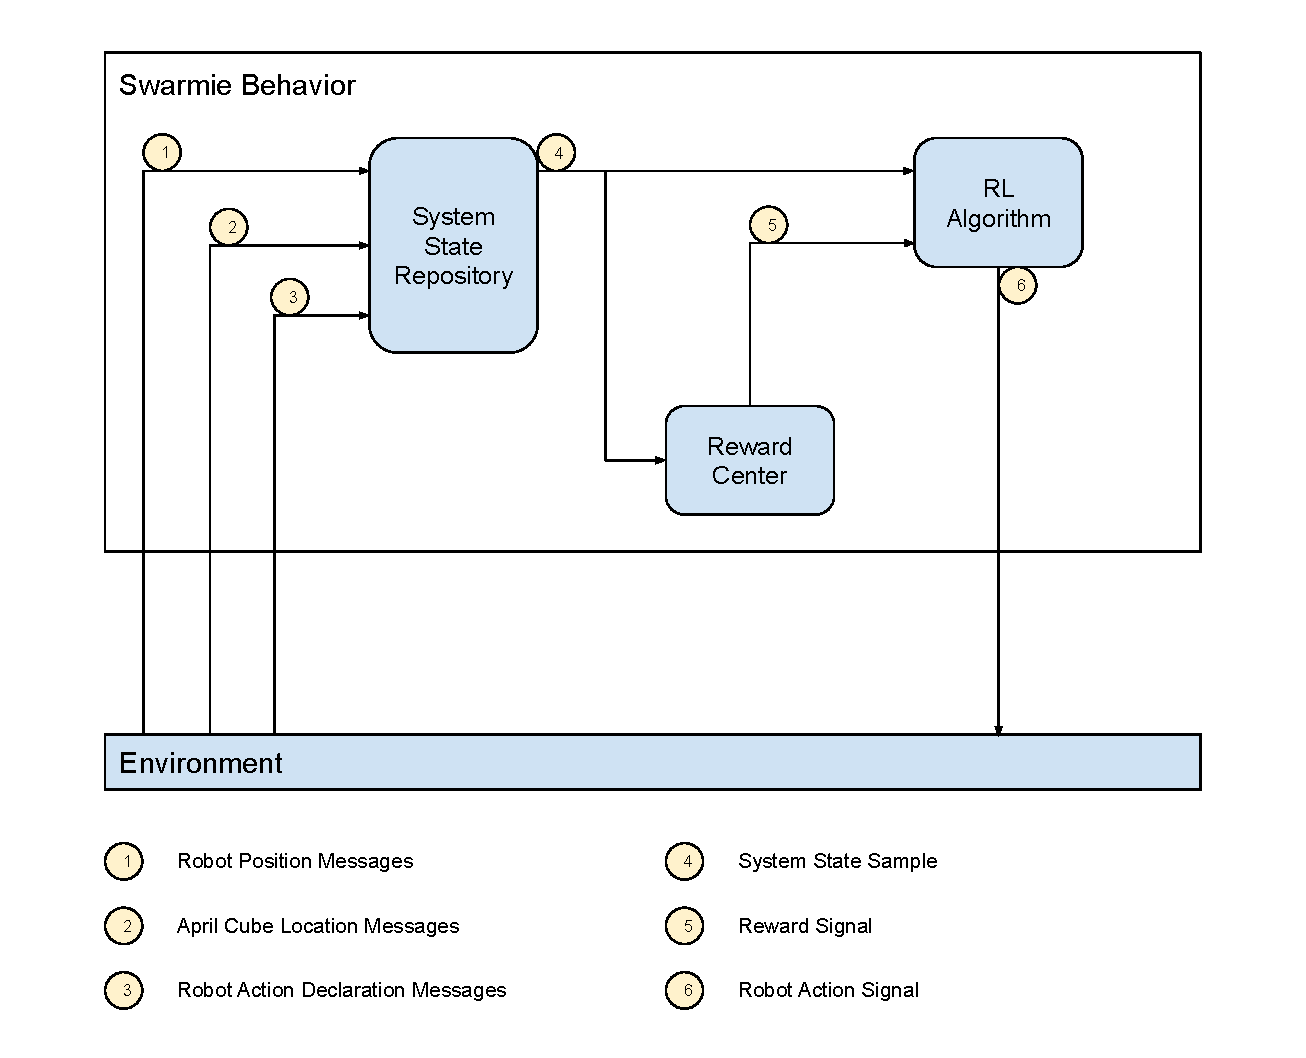
\includegraphics[width=0.5\textwidth]{images/architecture.pdf}
  \caption{High-level architectural diagram depicting how the RL algorithm integrates into the overall solution, including the types of information that flow into and out of the Swarmie behavior component.}
  \Description{High-level architectural diagram for the Swarmies RL solution.}
  \label{fig:architecture}
\end{figure}

Among other things, Figure \ref{fig:architecture} makes clear the kind of information that the behavior component requires in order to properly operate. A fuller description of these information types follows:

\begin{enumerate}
  \item \textbf{Robot Position Messages} - The system expects to be notified of the position of every Swarmie robot in the simulation on a regular basis, including the position of the robot hosting the behavior component instance.
  \item \textbf{April Cube Location Messages} - As Swarmie robots scan the competition area with their built-in camera, a separate component does enough processing on the incoming images in order to identify April Tags. Some of these tags are attached to April Cubes, and it is those kind of notifications that this message flow represents.
  \item \textbf{Robot Action Declaration Messages} - When a Swarmie makes an action decision, it publishes its intent for the benefit of other robots. Doing so helps maintain coherence within the ``robot busy'' indicators in the system state samples (see Section \ref{subsec:state_space}).
\end{enumerate}

Figure \ref{fig:architecture} also depicts the kind of information flow typical in Reinforcement Learning (RL) implementations, including system state samples (see Section \ref{subsec:state_space}), action results (see Section \ref{subsec:action_space}), and reward signals (see Section \ref{subsec:reward_signal}).

As far as the action results produced by the RL policy function, they are eventually post-processed into a form suitable for use with the rest of the NASA Swarmathon code base.

The ``System State Repository'' is a stateful component that retains information pertaining to last known Swarmie locations, declared actions, and April Cube sightings. The aforementioned subcomponent uses this cached information in order to maintain system state, and provide it to the Swarmie behavior component on demand. Both the RL algorithm and ``Reward Center'' benefit from this service.

\section{Experimental Results}\label{sec:results}
Results discussion.

\section{Conclusion}\label{sec:conclusion}
Final conclusion.

\bibliographystyle{ACM-Reference-Format}
\bibliography{swarmies_rl}

\end{document}
